\documentclass[aps,pre,reprint,twocolumn,nofootinbib,superscriptaddress]{revtex4-2}

\usepackage{amsmath,amssymb,amsthm}
\usepackage{graphicx}
\usepackage{bm}
\usepackage{xurl}
\usepackage{hyperref}

\hypersetup{
    pdfauthor={Taishi Namba},
    pdftitle={A resolution gap for the coarse-grained arrow of time in nonlinear Hamiltonian flows},
    pdfkeywords={coarse-graining, arrow of time, Fisher information, Tweedie formula, Cramer-Rao inequality, Gaussian mixtures},
    hidelinks
}

\newtheorem{theorem}{Theorem}
\newtheorem{proposition}[theorem]{Proposition}
\newtheorem{lemma}[theorem]{Lemma}
\newtheorem{corollary}[theorem]{Corollary}
\newtheorem*{gapconjecture}{Resolution-gap conjecture}
\newtheorem{observation}{Numerical result}
\theoremstyle{remark}
\newtheorem*{remark}{Remark}

\newcommand{\Sym}{\operatorname{Sym}}
\newcommand{\tr}{\operatorname{tr}}
\newcommand{\Cov}{\operatorname{Cov}}
\newcommand{\Var}{\operatorname{Var}}
\newcommand{\E}{\mathbb{E}}

\begin{document}

\title{A resolution gap for the coarse-grained arrow of time in nonlinear Hamiltonian flows}

\author{Taishi Namba}
\email{neginyan@gmail.com}
\affiliation{Independent Researcher, Atsugi, Kanagawa, Japan}

\date{\today}

\begin{abstract}
Gaussian coarse-graining at resolution $\sigma$ turns the conserved Gibbs entropy of a Hamiltonian ensemble into a coarse-grained entropy $S_C$. For an isotropic resolution that coarsens at rate $r = \dot\sigma/\sigma$, every state has a critical rate $R$ such that $dS_C/dt \geq 0$ if and only if $r \geq R$. For linear flows the supremum of $R$ over all states equals $\kappa$, the largest symmetric strain rate of the flow, and it has been conjectured that $R \leq \kappa$ for every state of a nonlinear flow. Here we derive an exact decomposition of $R$ into a law term, a covariance between the local Fisher matrix of the coarse-grained density and the local strain, and a posterior Stein defect. It shows that a violation of the conjecture requires either regions in which the local Fisher matrix has a negative eigenvalue, or a positive Stein defect. We prove the conjecture for all Gaussian states, in any dimension. For flows with one degree of freedom the best Gaussian state is a zero-width segment through the point of maximal strain, and the resolution gap of Gaussian states is $\kappa - R = 2\sqrt{2\beta\kappa}\,\sigma + O(\sigma^2)$, where $\beta$ measures how fast the strain decreases away from its maximum; we prove this exactly for the pendulum and for quadratic strain, and as an upper bound on the gap in general. For the pendulum the gap is $\sigma - \tfrac78\sigma^2 + \tfrac{65}{96}\sigma^3 - \cdots$, with exact rational coefficients. Gaussian states are not extremal: mixtures arranged as a fan of segments that cross at the point of maximal strain exceed the best Gaussian state by about $5\%$ of its gap, and in a flow whose stretching direction rotates, bent needles that follow the rotation reduce the gap by about $40\%$. In every case examined the gap remains proportional to $\sigma$. For the pendulum we prove, from a weighted Cram\'er--Rao inequality, a state-wise lower bound $\kappa - R \geq \Theta'\sigma/(1+\Theta'\sigma/2) - \tilde\varepsilon - D$. It gives a uniform gap under explicit conditions, and on all 268 stored pendulum states with $\sigma \leq 10^{-2}$ it is at least $0.898\,\sigma$, against a smallest observed gap of $0.946\,\sigma$. A uniform gap would follow from a bound on how fast the coarse-grained Fisher matrix can vary along the contracting direction, together with control of the valleys and of the Stein defect. All statements and numbers are reproduced by openly available code and are cross-checked by independent numerical methods.
\end{abstract}


\maketitle

\section{Introduction}
\label{sec:intro}

The Gibbs entropy of a Hamiltonian ensemble is constant, and the growth of entropy is commonly attributed to coarse-graining~\cite{gibbs1902,ehrenfest1912,wehrl1978,lebowitz1993}. In a previous paper~\cite{namba2026arrow} we asked when Gaussian coarse-graining guarantees that the coarse-grained entropy $S_C$ does not decrease for \emph{every} initial ensemble. For an isotropic window of width $\sigma(t)$ the answer is governed by a competition of two rates: the rate $r = \dot\sigma/\sigma$ at which the observer's resolution coarsens, and the rate at which the flow stretches phase space. For linear flows the coarse-grained entropy is non-decreasing for every state if and only if $r \geq \kappa$, the largest eigenvalue of the symmetric part of the flow's Jacobian. For nonlinear flows, with $\kappa$ the supremum of the symmetric strain rate, we proved partial results and stated the following conjecture: $r \geq \kappa$ implies $dS_C/dt \geq 0$ for every state~\cite{namba2026arrow}.

It is convenient to attach to each state a \emph{critical rate} $R$, defined so that $dS_C/dt \geq 0$ if and only if $r \geq R$ (Sec.~\ref{sec:decomposition}). The conjecture then reads $R \leq \kappa$ for every state. In this paper we study $R$ for nonlinear flows in detail. Our results are of three kinds.

\emph{Exact structure.} We derive an exact decomposition of $R$ into a law term, which never exceeds $\kappa$, a covariance between the local Fisher matrix $H(y) = -\nabla^2\ln\rho_C(y)$ of the coarse-grained density and the locally averaged strain, and a posterior Stein defect (Proposition~\ref{prop:decomposition}). It implies that the conjecture can fail only where $H$ has a negative eigenvalue, or through the Stein defect (Corollary~\ref{cor:where}).

\emph{Theorems.} We prove $R \leq \kappa$ for all Gaussian states in any dimension (Theorem~\ref{thm:gaussian}). For flows with one degree of freedom the best Gaussian state is a segment of zero width through the point of maximal strain, slightly tilted from the contracting direction. Its critical rate stays below $\kappa$ by a \emph{resolution gap} proportional to $\sigma$, $\kappa - R = 2\sqrt{2\beta\kappa}\,\sigma + O(\sigma^2)$, where $\beta$ measures how fast the strain decreases away from its maximum (Sec.~\ref{sec:best}). We prove this exactly for the pendulum, where the gap is a series with exact rational coefficients, and for quadratic strain, where it has a closed form; for general one-degree-of-freedom flows we prove it as an upper bound on the gap. Finally, from a weighted Cram\'er--Rao inequality we prove a lower bound on $\kappa - R$ for every state of the pendulum (Theorem~\ref{thm:statewise}).

\emph{Numerical results and a sharpened conjecture.} A natural guess, that no state beats the best Gaussian state, is false: mixtures arranged as a fan of segments crossing at the point of maximal strain gain about $5\%$ of the gap, and in a flow whose stretching direction rotates, bent needles that follow the rotation gain about $40\%$ (Sec.~\ref{sec:mixtures}). In more than two thousand states, including adversarial searches, the gap never closed and remained proportional to $\sigma$. This leads to the conjecture that $\kappa - R \geq c\,\sigma$ uniformly (Sec.~\ref{sec:evidence}), which would imply the original conjecture. We identify what prevents our state-wise bound from becoming uniform: mainly a bound on how fast the coarse-grained Fisher matrix can vary along the contracting direction, and in addition control of the valleys and of the Stein defect.

The physical picture behind these results is simple. The coarse-grained density cannot be sharper than the window, $H \preceq I/\sigma^2$. To see the full strain $\kappa$, an ensemble must be sharp across the stretching direction at the point of maximal strain; to be sharp across one direction it must be long along the other, and its ends then leave the point of maximal strain. The finite resolution therefore protects the arrow of time by a margin proportional to the resolution itself.

Every analytical statement and number in this paper is checked by openly available code (Data and Code Availability), and the central numbers were reproduced by independent numerical methods (Appendix~\ref{app:methods}).

\section{Critical rate and an exact decomposition}
\label{sec:decomposition}

\subsection{Setting}
We use the setting of Ref.~\cite{namba2026arrow}. Phase space is $\mathbb R^d$, $d = 2n$, with dimensionless canonical coordinates $z = (q,p)$, and $\dot z = f(z)$ is a Hamiltonian flow, so that $\nabla\cdot f = \tr Df = 0$. Let $X \sim \rho_t$ be the fine-grained state and $Y = X + \sigma Z$ with $Z \sim \mathcal N(0,I)$ independent of $X$. The coarse-grained density $\rho_C$ is the density of $Y$ and $S_C = h(Y)$ its differential entropy. We write $s = \nabla\ln\rho_C$ for the score, $F = \E[s(Y)s(Y)^{\mathsf T}]$ for the Fisher information matrix, and
\begin{equation}
H(y) = -\nabla^2\ln\rho_C(y)
\label{eq:H}
\end{equation}
for the \emph{local} Fisher matrix. Throughout we assume the regularity needed for the integrations by parts below and finite moments of the quantities involved ($\E\|Df(X)\|$, $\E[|f(X)|\,|X|]$ and, in Sec.~\ref{sec:bound}, fourth posterior moments); then $\E[H(Y)] = F$. The symmetric strain rate is $\kappa = \sup_z\lambda_{\max}[\Sym Df(z)]$.

For an isotropic window that coarsens at rate $r = \dot\sigma/\sigma$, Lemma~1 of Ref.~\cite{namba2026arrow} gives $dS_C/dt = r\,\sigma^2\tr F + \Sigma$ with $\Sigma = -\E[s(Y)\cdot f(X)]$. We define the \emph{critical rate} of the state,
\begin{equation}
R = -\frac{\Sigma}{\sigma^2\tr F}, \qquad \frac{dS_C}{dt} = \sigma^2\tr F\,(r - R).
\label{eq:R}
\end{equation}
The coarse-grained entropy of the state does not decrease if and only if $r \geq R$. Conjecture~1 of Ref.~\cite{namba2026arrow} states that $R \leq \kappa$ for every state, every $\sigma > 0$ and every Hamiltonian flow with $\kappa < \infty$. For linear flows $\dot z = Bz$ one has $R = \tr(F\Sym B)/\tr F \leq \kappa$, and the supremum over states equals $\kappa$~\cite{namba2026arrow}.

Two facts about Gaussian smoothing are used throughout. First, $\Sigma = \E[\tr\Cov(f(X),X\,|\,Y)]/\sigma^2$ (Lemma~2 of Ref.~\cite{namba2026arrow}). Second, differentiating Tweedie's formula for the posterior mean~\cite{efron2011}, $\E[X\,|\,y] = y + \sigma^2 s(y)$, once more with respect to $y$ gives the second-order formula
\begin{equation}
\Cov(X\,|\,Y = y) = \sigma^2 I - \sigma^4 H(y).
\label{eq:tweedie2}
\end{equation} Because the left-hand side is positive semidefinite,
\begin{equation}
H(y) \preceq \sigma^{-2} I \qquad \text{for every } y .
\label{eq:Hbound}
\end{equation}
The coarse-grained density can nowhere be sharper than the window. Equation~\eqref{eq:Hbound} is the Euclidean form of the matrix Harnack estimate for the heat equation~\cite{hamilton1993}, with heat-kernel time $\sigma^2/2$. It bounds $H$ from above only: between separated components $H$ can be strongly negative.

\subsection{Decomposition}
Let $G(y) = \Sym\E[Df(X)\,|\,Y = y]$ be the locally averaged strain seen at $y$, and $\bar G = \E[G(Y)] = \Sym\E_{\rho_t}[Df]$ its average over the state. Define the posterior Stein defect
\begin{equation}
\Delta(y) = \Cov(f(X),X\,|\,y) - \E[Df(X)\,|\,y]\,\Cov(X\,|\,y),
\label{eq:defect}
\end{equation}
which vanishes when the posterior law of $X$ given $Y = y$ is Gaussian, by Stein's lemma~\cite{stein1981}.

\begin{proposition}[Decomposition of the critical rate]
\label{prop:decomposition}
For every state,
\begin{equation}
R = \underbrace{\frac{\tr(F\bar G)}{\tr F}}_{L}
+ \underbrace{\frac{\E\tr\!\left[(H(Y) - F)\,G(Y)\right]}{\tr F}}_{C}
+ \underbrace{\left(-\frac{\E\tr\Delta(Y)}{\sigma^4\tr F}\right)}_{D} .
\label{eq:decomposition}
\end{equation}
The law term satisfies $L \leq \lambda_{\max}(\bar G) \leq \kappa$.
\end{proposition}

\begin{proof}
Insert Eq.~\eqref{eq:defect} and Eq.~\eqref{eq:tweedie2} into $\Sigma = \E[\tr\Cov(f(X),X\,|\,Y)]/\sigma^2$:
$\Sigma = \E\tr\E[Df\,|\,Y] - \sigma^2\,\E\tr(H\,\E[Df\,|\,Y]) + \E\tr\Delta/\sigma^2$.
The first term is $\E[\nabla\cdot f(X)] = 0$. Since $H$ is symmetric, $\tr(H\,\E[Df\,|\,Y]) = \tr(H\,G)$. Hence $R = \E\tr(HG)/\tr F + D$, and writing $H = F + (H - F)$ with $\E\tr(FG(Y)) = \tr(F\bar G)$ gives Eq.~\eqref{eq:decomposition}. Because $F \succeq 0$, $\tr(F\bar G) \leq \lambda_{\max}(\bar G)\tr F$, and $\lambda_{\max}(\bar G) \leq \E_{\rho_t}\lambda_{\max}(\Sym Df) \leq \kappa$ by convexity of $\lambda_{\max}$.
\end{proof}

The covariance term $C$ is positive when the coarse-grained density is sharper than average ($H \succ F$) where the local strain is strong. In words: the observer's focus sits where the flow stretches. The Stein defect $D$ measures how far the posterior laws are from Gaussian. For a single Gaussian state both vanish (Sec.~\ref{sec:gaussian}). Rewriting Eq.~\eqref{eq:decomposition} with $A(y) = \kappa I - G(y) \succeq 0$ gives a form that shows where the conjecture can fail.

\begin{corollary}[Where the conjecture can fail]
\label{cor:where}
For every state,
\begin{equation}
\kappa - R = \frac{\E\tr\!\left[H(Y)A(Y)\right]}{\tr F} - D,
\qquad A(y) = \kappa I - G(y) \succeq 0 .
\label{eq:where}
\end{equation}
If $H(y) \succeq 0$ for all $y$, then $R \leq \kappa + D$. A state with $R > \kappa$ therefore needs either a positive Stein defect or a region where $H$ has a negative eigenvalue whose direction meets large values of $A$.
\end{corollary}

\begin{proof}
Use $\E\tr H = \tr F$ in Eq.~\eqref{eq:decomposition}. If $H \succeq 0$, then $\tr(HA) \geq 0$ because $A \succeq 0$.
\end{proof}

Regions where $H$ has a negative eigenvalue are the ``valleys'' of $\ln\rho_C$, for example between overlapping components of a mixture. For one-degree-of-freedom flows with $f = (p, g(q))$, $\Sym Df = a(q)\,\mathrm{diag}(1,-1)$ in the rotated coordinates $v = (q+p)/\sqrt2$, $w = (q-p)/\sqrt2$, with
\begin{equation}
a(q) = \tfrac12\left(1 + g'(q)\right),
\label{eq:stretch}
\end{equation}
so that $G(y) = \bar a(y)\,\mathrm{diag}(1,-1)$ with $\bar a(y) = \E[a(X_q)\,|\,y]$. We call $v$ the stretching and $w$ the contracting direction. Equation~\eqref{eq:where} then reads
\begin{equation}
\kappa - R = \frac{\E\left[(\kappa - \bar a)H_{vv}\right] + \E\left[(\kappa + \bar a)H_{ww}\right]}{\tr F} - D .
\label{eq:where1d}
\end{equation}
For the pendulum, $g(q) = -\sin q$, $a(q) = (1-\cos q)/2 \in [0,1]$ and $\kappa = 1$, attained at the hyperbolic point $q = \pi$. Figure~\ref{fig:mechanism} shows $\bar a$, the local anisotropy of $H$, the valleys and the density of the covariance term for three pendulum states.

\begin{figure*}[t]
\centering
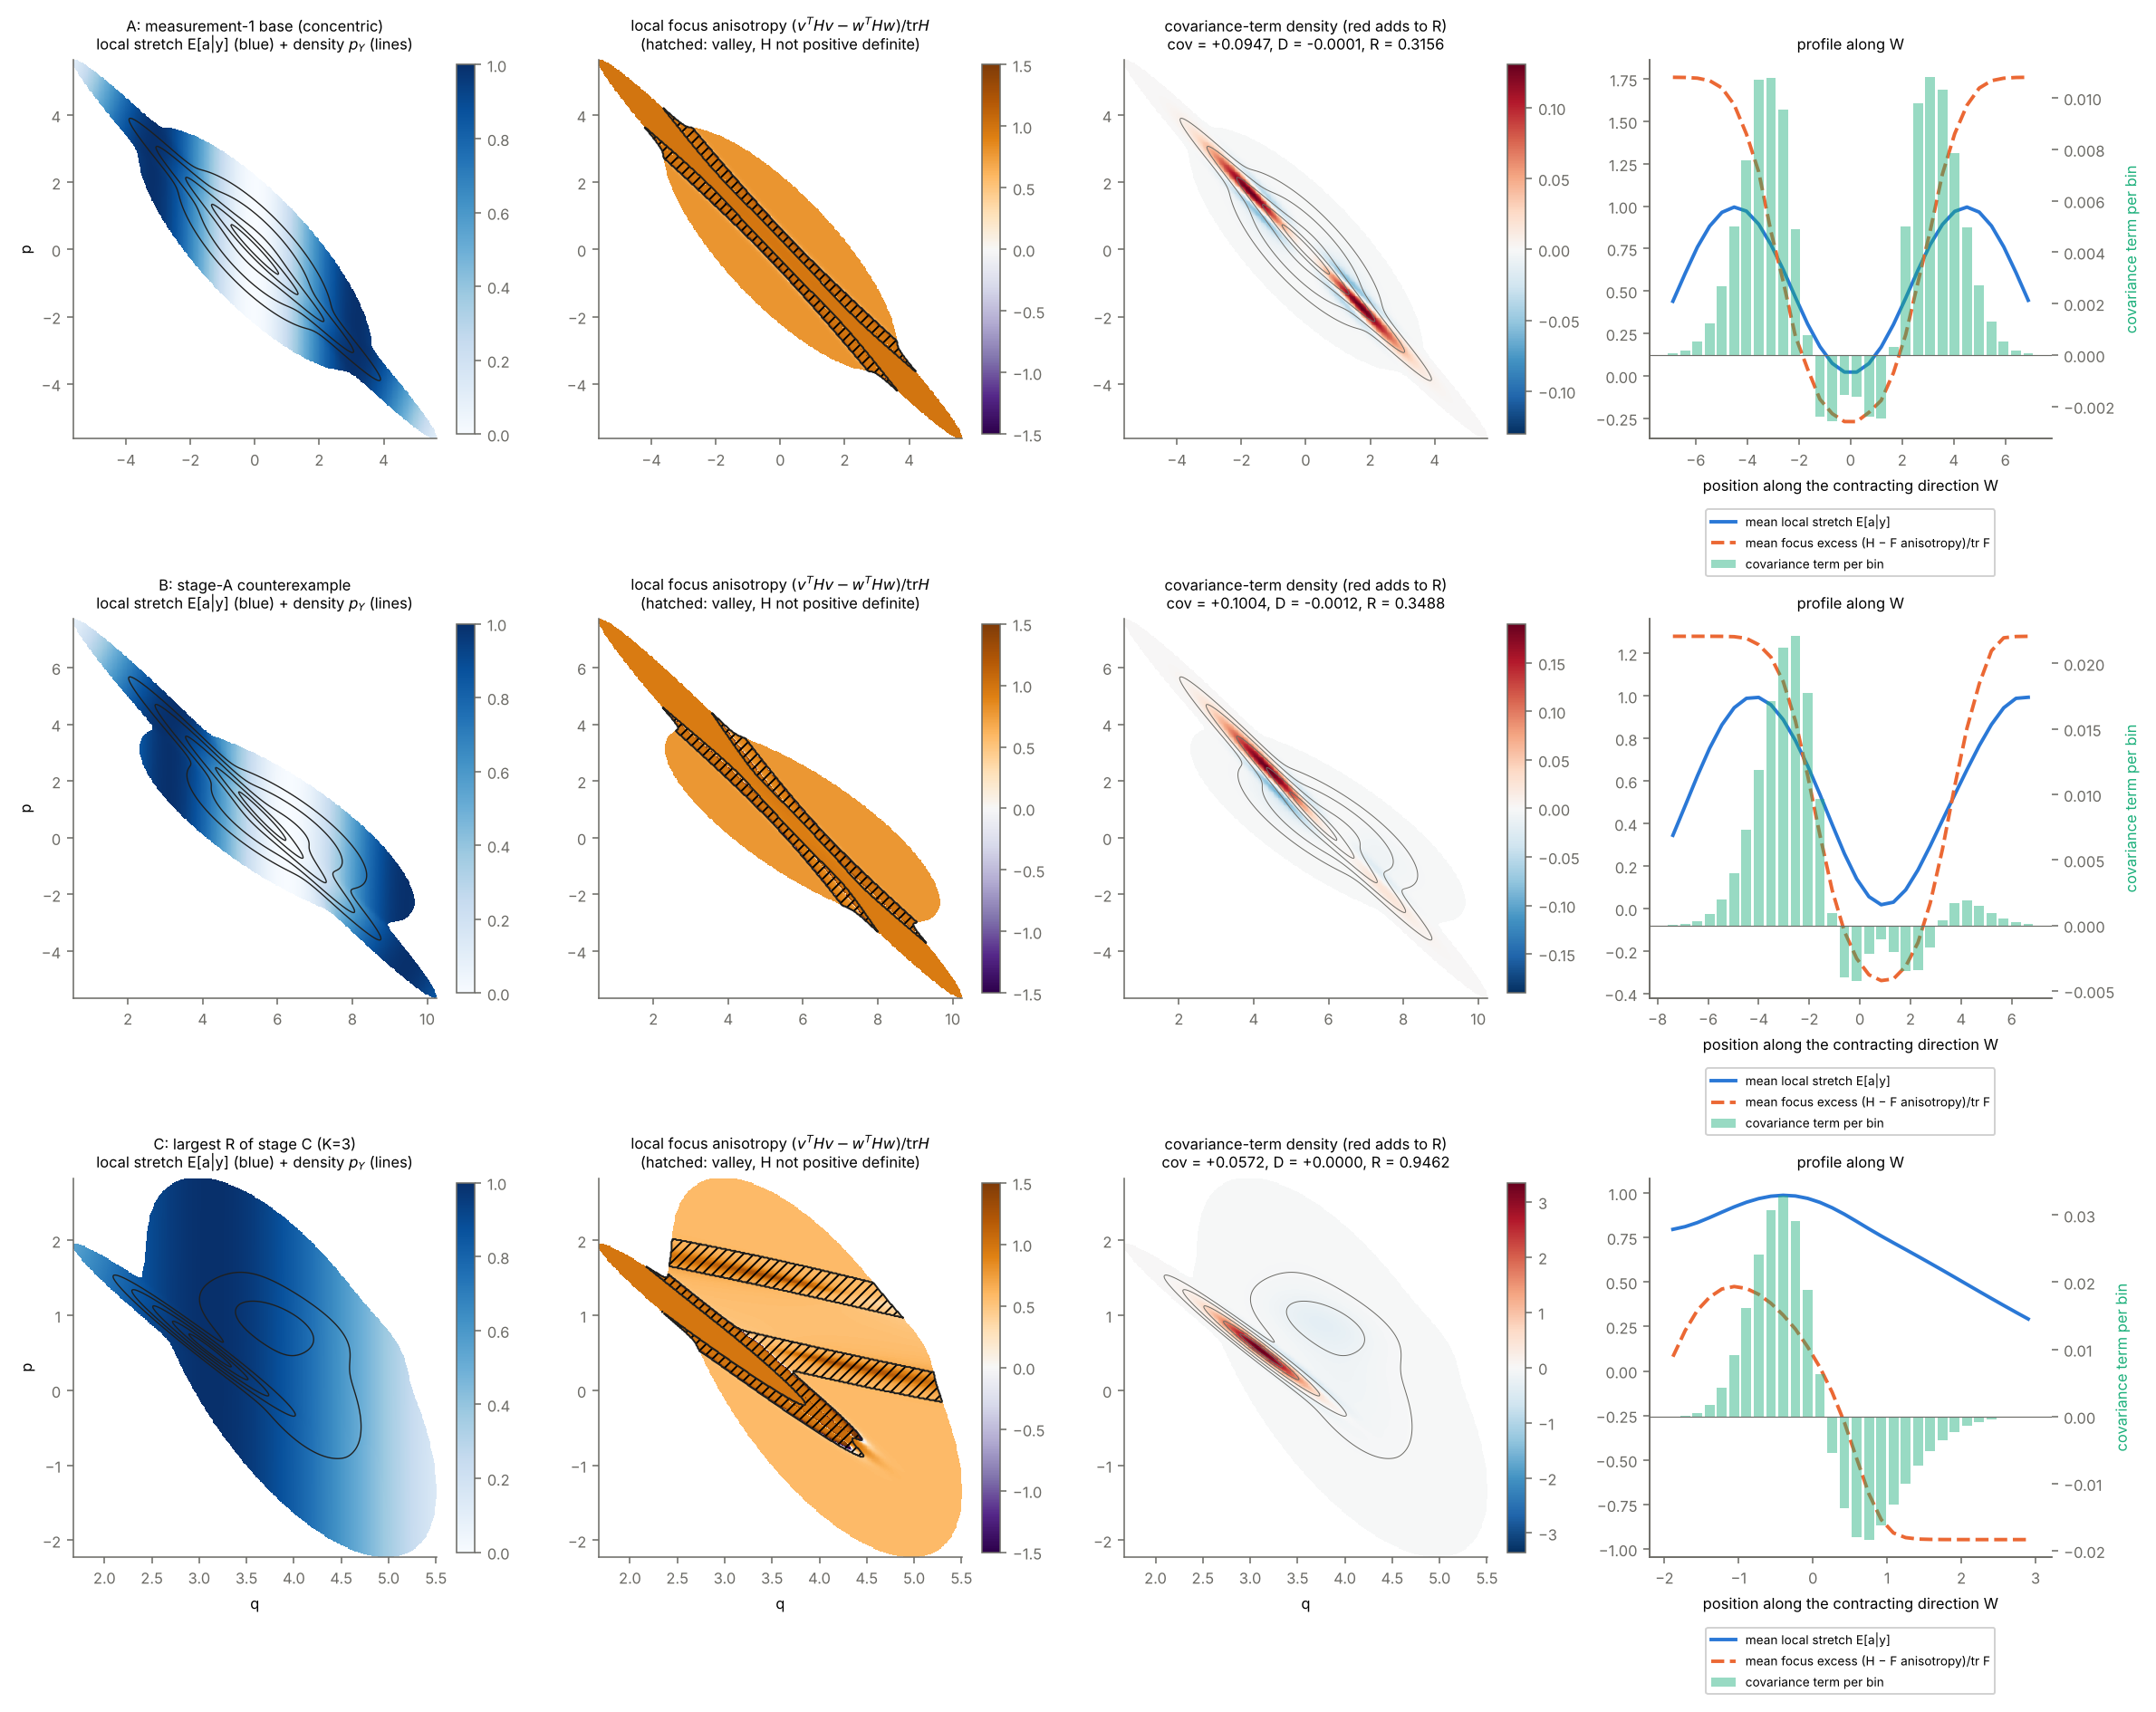
\includegraphics[width=0.95\textwidth]{figures/fig1_mechanism.png}
\caption{Mechanism of the covariance term for three pendulum states (rows). Left: local strain $\bar a(y)$ and coarse-grained density (contours). Second: local anisotropy of the focus $(v^{\mathsf T}Hv - w^{\mathsf T}Hw)/\tr H$; hatched regions are valleys, where $H$ has a negative eigenvalue. Third: density of the covariance term $C$ (red adds to $R$). Right: profile along the contracting direction. The covariance term is positive where the focus is sharp and the strain is strong.}
\label{fig:mechanism}
\end{figure*}

\section{Gaussian states}
\label{sec:gaussian}

\begin{theorem}[Gaussian states]
\label{thm:gaussian}
Let $\rho_t = \mathcal N(m,S)$ at some instant $t$. Then, for every $\sigma > 0$ and every Hamiltonian flow,
\begin{equation}
R = \frac{\tr(F\,\Sym\bar J)}{\tr F} \leq \lambda_{\max}(\Sym\bar J) \leq \kappa,
\label{eq:gaussian}
\end{equation}
where $\bar J = \E_{\rho_t}[Df]$ and $F = (S + \sigma^2 I)^{-1}$. Hence Conjecture~1 of Ref.~\cite{namba2026arrow} holds for all Gaussian states, in any dimension.
\end{theorem}

\begin{proof}
$Y$ is Gaussian with covariance $S + \sigma^2 I$, so $H(y) \equiv F = (S+\sigma^2I)^{-1}$ and $C = 0$. The posterior law of $X$ given $Y$ is Gaussian, so $\Delta = 0$ and $D = 0$. Proposition~\ref{prop:decomposition} gives $R = L$ with $\bar G = \Sym\bar J$.
\end{proof}

A direct proof uses Stein's lemma, $\E[f(X)(X-m)^{\mathsf T}] = \bar J S$, together with $\tr\bar J = 0$. This step is the statistical linearization used in Gaussian filtering~\cite{sarkka2013}: for Gaussian states, the coarse-grained entropy production equals that of the flow linearized with the averaged Jacobian $\bar J$. The theorem is instantaneous: a nonlinear flow does not preserve Gaussianity, and states at later times are covered only if they are again Gaussian.

Equation~\eqref{eq:gaussian} also shows what a Gaussian state needs in order to approach $\kappa$. The averaged strain $\lambda_{\max}(\Sym\bar J)$ must approach $\kappa$, so the state must be concentrated where the strain is maximal. And the Fisher matrix $F$ must be concentrated on the top eigenvector of $\Sym\bar J$, so the coarse-grained density must be sharp across the stretching direction and broad along the contracting one. Because $F \preceq \sigma^{-2}I$, the second requirement forces the state to be long, and a long state cannot stay where the strain is maximal. Section~\ref{sec:best} turns this tension into a quantitative gap.

\section{The best Gaussian state and the resolution gap}
\label{sec:best}

From now on we consider flows with one degree of freedom, $f = (p, g(q))$, that is, $H = p^2/2 + V(q)$ with $g = -V'$. Their strain is $a(q)\,\mathrm{diag}(1,-1)$ in the coordinates $(v,w)$ of Sec.~\ref{sec:decomposition}, with $a$ from Eq.~\eqref{eq:stretch}. We write $T = S + \sigma^2 I$ for the covariance of $Y$ and use $(v,w)$ components.

\begin{lemma}[Gaussian states of one-degree-of-freedom flows]
\label{lem:lambdaphi}
For $\rho_t = \mathcal N(m,S)$,
\begin{equation}
R = \lambda\,\varphi, \qquad \lambda = \E_{\rho_t}[a(X_q)], \qquad \varphi = \frac{T_{ww} - T_{vv}}{T_{ww} + T_{vv}} .
\label{eq:lambdaphi}
\end{equation}
\end{lemma}

\begin{proof}
By Theorem~\ref{thm:gaussian}, $R = \tr(F\bar G)/\tr F$ with $\bar G = \lambda\,\mathrm{diag}(1,-1)$ and $F = T^{-1}$. For a $2\times2$ matrix, $F_{vv} = T_{ww}/\det T$ and $F_{ww} = T_{vv}/\det T$.
\end{proof}

The two factors in Eq.~\eqref{eq:lambdaphi} are the two requirements of Sec.~\ref{sec:gaussian}: $\lambda$ is the strain felt by the state and $\varphi \in (-1,1)$ is the anisotropy of the observer's focus. The aspect factor $\varphi$ depends on $S$ only through $S_{vv}$ and $S_{ww}$, while $\lambda$ depends on $S$ through the variance $S_{qq} = (S_{vv} + 2S_{vw} + S_{ww})/2$ of $X_q$. At fixed $S_{vv}, S_{ww}$, $S_{qq}$ is smallest when $S_{vw} = -\sqrt{S_{vv}S_{ww}}$, a state of zero width: a straight segment whose direction is tilted from $w$ towards $-v$. If $\lambda$ decreases with $S_{qq}$, which is the case at the point of maximal strain, the supremum over Gaussian states is approached by states that tend to a segment of zero width; we admit such degenerate Gaussian states as limits and call them segments. Writing $x = \sqrt{2S_{qq}}$, which for a nearly $w$-aligned segment is close to its standard deviation along its length, the remaining optimization over the tilt can be done in closed form (Appendix~\ref{app:best}):
\begin{equation}
\max_{\text{tilt}}\varphi = \frac{x}{\sqrt{x^2 + 4\sigma^2}} .
\label{eq:phimax}
\end{equation}
This reduces the best Gaussian state to a maximization over one variable.

\begin{theorem}[Pendulum]
\label{thm:pendulum}
For the pendulum, $a(q) = (1-\cos q)/2$ and $\kappa = 1$. For every $\sigma > 0$ the supremum of $R$ over Gaussian states is
\begin{equation}
R^*(\sigma) = \sup_{x > 0}\;\frac{1 + e^{-x^2/4}}{2}\,\frac{x}{\sqrt{x^2 + 4\sigma^2}} .
\label{eq:Rstar}
\end{equation}
For $\sigma \leq \sigma_c = 0.93909\ldots$ it is attained at a finite $x$, by a zero-width segment centred at $q = \pi$, with standard deviation along its length close to $2\sqrt\sigma$, tilted from $w$ towards $-v$ by an angle close to $\sigma/4$. Its gap has the expansion
\begin{align}
1 - R^*(\sigma) &= \sigma - \frac78\sigma^2 + \frac{65}{96}\sigma^3 - \frac{61}{128}\sigma^4 \nonumber\\
&\quad + \frac{3151}{10240}\sigma^5 - \frac{8483}{46080}\sigma^6 + O(\sigma^7) .
\label{eq:series}
\end{align}
For $\sigma > \sigma_c$, $R^*(\sigma) = 1/2$ and is not attained.
\end{theorem}

The proof is in Appendix~\ref{app:best}. The coefficients in Eq.~\eqref{eq:series} were computed in exact rational arithmetic up to $\sigma^{11}$; the truncation error of the series equals the size of the next term, and through $\sigma^{11}$ it reproduces Eq.~\eqref{eq:Rstar} to $10^{-9}$ at $\sigma = 0.3$ (Fig.~\ref{fig:best}).

\begin{figure*}[t]
\centering
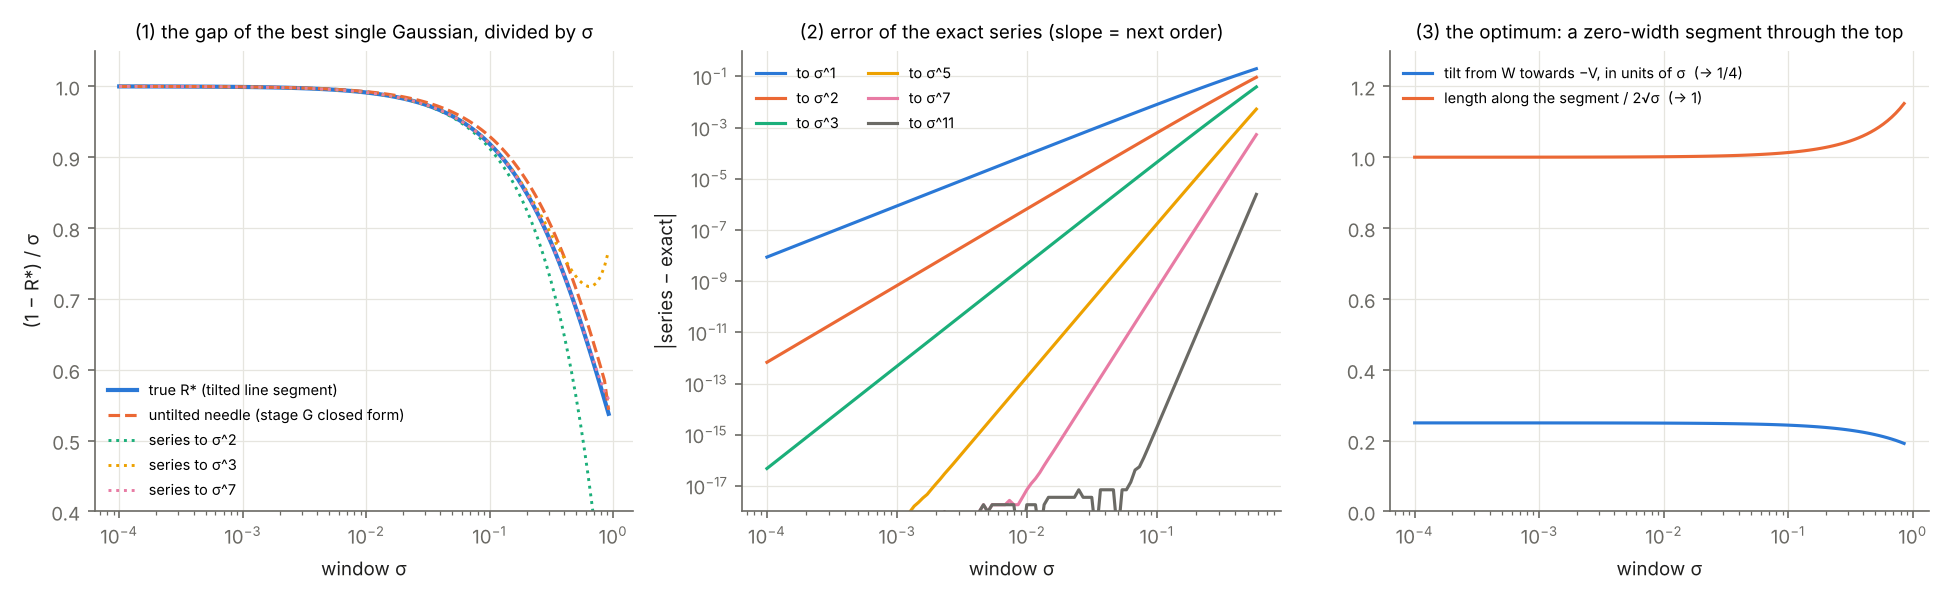
\includegraphics[width=0.95\textwidth]{figures/fig2_best_gaussian.png}
\caption{Best Gaussian state of the pendulum. (1) Gap $(1-R^*)/\sigma$ of the optimal tilted segment, of the untilted needle, and of truncations of the series~\eqref{eq:series}. (2) Error of the truncated series; the slope equals the next order. (3) Shape of the optimum: tilt from $w$ towards $-v$ in units of $\sigma$ ($\to1/4$) and length in units of $2\sqrt\sigma$ ($\to1$).}
\label{fig:best}
\end{figure*}

For a strain that is exactly quadratic about its maximum the optimization can be done completely.

\begin{theorem}[Quadratic strain]
\label{thm:quadratic}
Let $a(q) = \kappa - b(q - q_*)^2$ with $\kappa, b > 0$, and let $\varepsilon = \sigma\sqrt{b/\kappa}$. Among Gaussian states with $\varphi \geq 0$,
\begin{equation}
\frac{R^*}{\kappa} = \left(1 - \frac{\varepsilon\nu}{2}\right)\sqrt{\frac{\nu}{\nu + 4\varepsilon}},
\qquad \nu = \sqrt{4 + 9\varepsilon^2} - 3\varepsilon ,
\label{eq:quadratic}
\end{equation}
attained by the zero-width segment centred at $q_*$ with $S_{qq} = \tfrac12\sigma\nu\sqrt{\kappa/b}$. In particular $1 - R^*/\kappa = 2\varepsilon - \tfrac52\varepsilon^2 + \tfrac74\varepsilon^3 - \tfrac18\varepsilon^4 - \tfrac{53}{64}\varepsilon^5 + O(\varepsilon^6)$.
\end{theorem}

The restriction $\varphi \geq 0$ selects states whose focus is sharper across $v$ than across $w$, the relevant ones near a maximum of $a$. It is needed because for such polynomial potentials $|a|$ is unbounded and the global strain rate is infinite; here $\kappa$ denotes the maximum of $a$, not the supremum of $|a|$. The double well $g = q - q^3$ ($a = 1 - \tfrac32 q^2$) and the quartic oscillator $g = -q^3$ ($a = \tfrac12 - \tfrac32q^2$) are exactly of this form. Both theorems share the same leading behaviour, which we state for a general maximum.

\begin{proposition}[Resolution gap of Gaussian states]
\label{prop:gap}
Let $a$ be of at most polynomial growth and four times continuously differentiable near a non-degenerate maximum $\kappa = a(q_*) > 0$ with $a''(q_*) = -2b$, and let $\beta = b/2$, the rate at which the strain decreases quadratically along the contracting direction $w$ through the maximum. Let $R^*(\sigma)$ be the supremum of $R$ over Gaussian states with $\varphi \geq 0$. Then
\begin{equation}
\kappa - R^*(\sigma) \leq 2\sqrt{2\beta\kappa}\,\sigma + O(\sigma^2) .
\label{eq:gap}
\end{equation}
Equality holds to this order whenever $\E_\rho[a(X_q)] \leq \Lambda(S_{qq})$ for all Gaussian states $\rho$ with $\varphi \geq 0$, for a non-increasing function $\Lambda$ with $\Lambda(s) = \kappa - bs + O(s^2)$ as $s \to 0$ and $\sup_{s \geq s_0}\Lambda(s) < \kappa$ for every $s_0 > 0$. This condition holds for the pendulum, with $\Lambda(s) = (1 + e^{-s/2})/2$, $\beta = 1/8$ and coefficient $1$, and for quadratic strain (Theorem~\ref{thm:quadratic}).
\end{proposition}

The proof (Appendix~\ref{app:best}) balances two losses. A segment with standard deviation $x$ along its length loses $\tfrac12 b x^2$ of strain because its ends leave the maximum, and loses a fraction $2\sigma^2/x^2$ of focus because the window has width $\sigma$. The sum $\tfrac12 b x^2 + 2\kappa\sigma^2/x^2$ is smallest for $x^2 = 2\sigma\sqrt{\kappa/b}$, where both losses equal $\sqrt{2\beta\kappa}\,\sigma$. The gap is linear in $\sigma$, although the window enters the loss of focus quadratically, because the optimal length grows like $\sqrt\sigma$.

Figure~\ref{fig:flows} (panel 1) shows the gap for four flows: the pendulum and the double well and quartic oscillator, which are covered by Theorems~\ref{thm:pendulum} and~\ref{thm:quadratic}, and the twist flow $H = \tfrac12\ln(1+q^2+p^2)$. The numerically optimized Gaussian states agree with $2\sqrt{2\beta\kappa}$ to $10^{-7}$ after extrapolation to $\sigma\to0$: coefficients $1$, $\sqrt6$, $\sqrt3$ and $\sqrt3/2$. The twist flow is not of the form $f = (p,g(q))$: its maximal strain $\kappa = 1/4$ is attained on the circle $q^2+p^2 = 1$, and its stretching direction rotates along the contracting direction. For it, $\beta = 3/8$ is the sum of the decrease of the strain with radius ($1/8$) and of the turning of the stretching direction ($1/4$). Proposition~\ref{prop:gap} is proved here only for $f = (p,g(q))$; the twist flow is a numerical observation.

\section{Mixtures beat the best Gaussian state}
\label{sec:mixtures}

Since Gaussian states are often extremal for information inequalities~\cite{stam1959,cover2006}, it is natural to ask whether $R \leq R^*(\sigma)$ for every state. It is not. We measure the advantage of a state over the best Gaussian state at the same resolution, in units of the Gaussian gap, by
\begin{equation}
g^* = \frac{R - R^*(\sigma)}{1 - R^*(\sigma)} .
\label{eq:gstar}
\end{equation}

\begin{observation}[Fans of segments]
\label{obs:fan}
For the pendulum there are Gaussian mixtures with $g^* > 0$ at every $\sigma$ examined ($10^{-5} \leq \sigma \leq 0.3$). Adversarial searches found $g^* = 0.031$, $0.037$ and $0.043$ for $K = 2, 3, 4$ components at $\sigma = 10^{-3}$, and $g^* = 0.053$ for $K = 8$. The optimal states are fans of thin segments that all pass through the hyperbolic point $q = \pi$, with slightly different tilts and lengths (Fig.~\ref{fig:fan}). A fan described by continuous profiles of weight, length, thickness and offset over the tilt angle reaches $g^* = 0.0478$, unchanged between $20$ and $80$ segments. The advantage is scale invariant: rescaling a state from $\sigma = 10^{-3}$ to $10^{-5}$ changes $g^*$ by less than $2\times10^{-3}$. In every case $R < 1$. For $\sigma \leq 10^{-2}$ the gap satisfies $(1-R)/\sigma \geq 0.946$; at larger $\sigma$ the gaps of all states, including the best Gaussian one, fall below $\sigma$ through the higher-order terms of Eq.~\eqref{eq:series}, and the advantage of mixtures stays at a few percent of the Gaussian gap (Fig.~\ref{fig:fan}, panel 3).
\end{observation}

The violation of $R \leq R^*$ was confirmed by three independent evaluations: closed-form posterior moments with quadrature on four grids, Gauss--Hermite quadrature of the posterior expectations, and a direct summation over nodes of the fine-grained state that uses no closed forms. In addition, the coarse-grained entropy was computed directly on a grid and differentiated in time, without using any of the identities of Sec.~\ref{sec:decomposition}; for two of the violating states ($\sigma = 0.1$ and $0.3$) this reproduced $R - R^* = 0.002390$ and $0.005528$ to $10^{-7}$ (Appendix~\ref{app:methods}).

The mechanism is visible in the decomposition~\eqref{eq:decomposition}. Each component of the fan is, on its own, below the best Gaussian state. In the mixture the components overlap only near the common point $q = \pi$, so the focus of the coarse-grained density concentrates where the strain is maximal. A single segment spreads its focus uniformly over its length and cannot do this. The gain comes from the covariance term $C$; the Stein defect is negligible ($D \approx 3\times10^{-7}$ for the best $K = 4$ state).

\begin{figure*}[t]
\centering
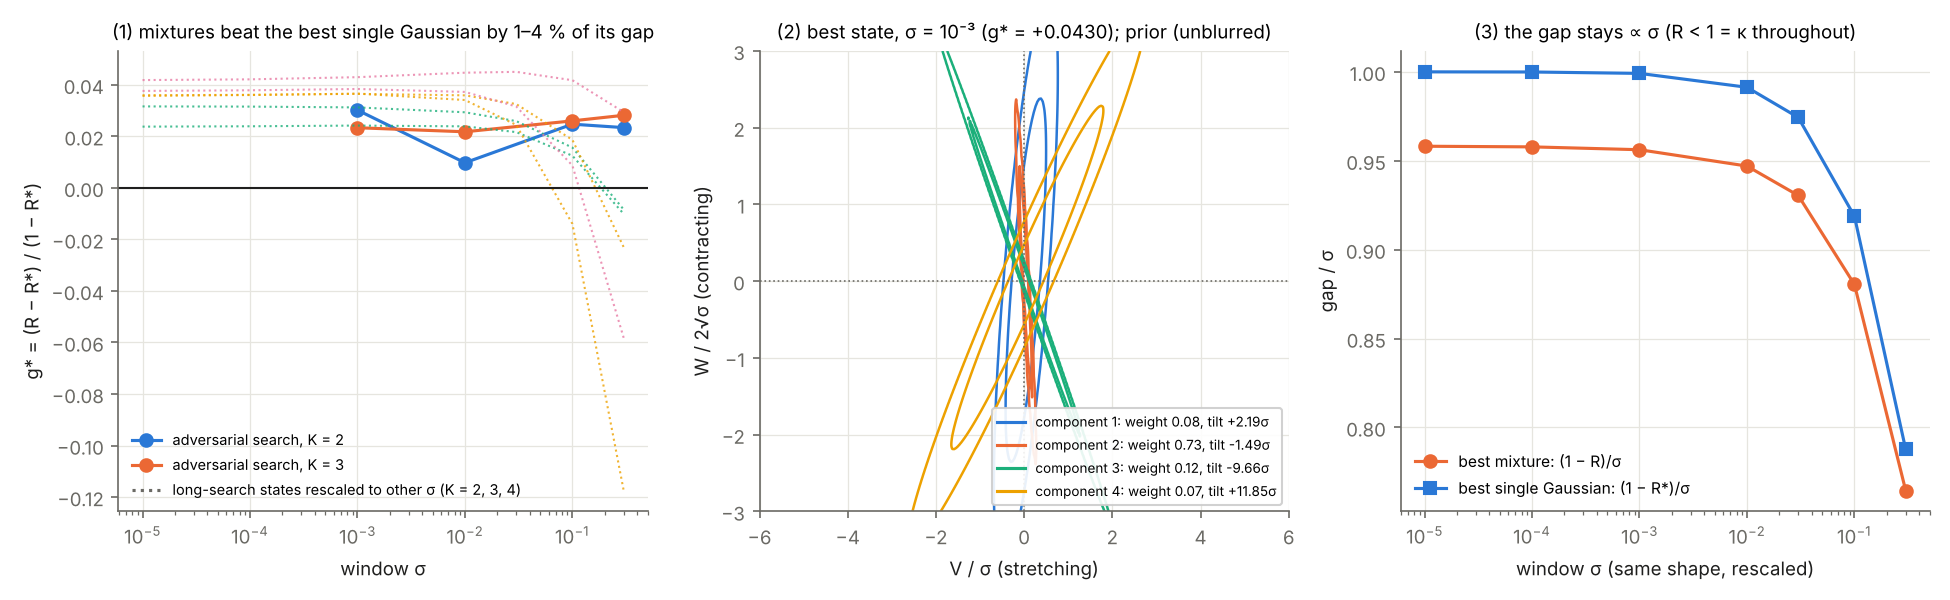
\includegraphics[width=0.95\textwidth]{figures/fig3_fan.png}
\caption{Mixtures that beat the best Gaussian state (pendulum). (1) Advantage $g^*$ of adversarially optimized mixtures with $K = 2$ and $3$ components, and of long searches rescaled to other $\sigma$. (2) The best state at $\sigma = 10^{-3}$ ($K = 4$): four thin components crossing at $q = \pi$, shown in units of $\sigma$ across and $2\sqrt\sigma$ along. (3) The gap stays proportional to $\sigma$ for the best mixture and for the best Gaussian state.}
\label{fig:fan}
\end{figure*}

In the twist flow, where the stretching direction rotates, the advantage is much larger.

\begin{observation}[Bent needles]
\label{obs:bent}
For the twist flow $H = \tfrac12\ln(1+q^2+p^2)$, $\kappa = 1/4$, the best Gaussian state has gap $(\kappa - R^*)/\sigma \to \sqrt3/2 \approx 0.866$. Mixtures reach $0.525$ ($K = 8$), and a needle bent along an arc reaches $0.509$. The optimal curvature, $0.709$ to $0.714$ in four independent optimizations, equals the rate $1/\sqrt2$ at which the stretching direction turns along the contracting direction, and the gap agrees with $2\sqrt{2\beta_{\rm eff}\kappa} = 1/2$ for $\beta_{\rm eff} = 1/8$, the value of $\beta$ without the turning contribution. The gap is scale invariant ($\sigma = 10^{-4}$ to $10^{-2}$) and remains proportional to $\sigma$.
\end{observation}

We reproduced the gap of the best $K = 8$ twist state by a direct summation over nodes of each component, transported by the exact flow, with the entropy computed on a grid and differentiated in time: $R = 0.24946085749$ against $0.24946085792$ from the closed-form evaluator.

The bent needle shows that a state can follow a rotating frame of stretching directions and so remove the part of $\beta$ that comes from the rotation. What cannot be removed is the decrease of the strain itself away from its maximum, which is why the gap stays linear in $\sigma$. For the double well and the quartic oscillator, where the stretching direction is fixed, short searches found only small advantages ($g^* \leq 0.02$), comparable to the pendulum fan.

\section{A state-wise lower bound on the gap}
\label{sec:bound}

We now bound $\kappa - R$ from below for every state of the pendulum, using only exact identities, an elementary inequality for the strain, the bound~\eqref{eq:Hbound}, and a weighted Cram\'er--Rao inequality~\cite{rao1945,cramer1946} along the contracting direction. Let $\delta = X_q - \pi$ and
\begin{align}
\gamma(y) &= 1 - \bar a(y) = \E[\sin^2(\delta/2)\,|\,y] \in [0,1], \\
\omega(y) &= \sigma^2\,[H_{vv}(y)]_+ \in [0,1], \\
u(y) &= \sqrt2\,\left(\E[X_q\,|\,y] - \pi\right),
\end{align}
the local strain deficit, the focus weight across the stretching direction, and the signed offset of the posterior mean from the hyperbolic point, scaled by $\sqrt2$. Let $j = \E[\omega(Y)]$, $s_w$ the $w$ component of the score, and $[x]_\pm = \max(\pm x, 0)$. Define
\begin{equation}
\Theta' = \frac{|\E[\omega u s_w]|}{j}\sqrt{\frac{F_{ww}}{\E[\omega s_w^2]}},
\label{eq:Theta}
\end{equation}
\begin{align}
\tilde\varepsilon = \frac{1}{\tr F}\Bigl\{&\sigma^{-2}\,\E\!\left[\omega\left(\tfrac{1}{48}\E[\delta^4|Y] - \tfrac14\Var(X_q|Y)\right)\right] \nonumber\\
&+ \E\!\left[\gamma\,[H_{vv}]_-\right] + \E[\gamma H_{ww}]\Bigr\}.
\label{eq:epstilde}
\end{align}

\begin{theorem}[State-wise lower bound]
\label{thm:statewise}
For every state of the pendulum and every $\sigma > 0$,
\begin{equation}
1 - R \;\geq\; \frac{\Theta'\sigma}{1 + \Theta'\sigma/2} - \tilde\varepsilon - D ,
\label{eq:statewise}
\end{equation}
with $D$ the Stein defect of Proposition~\ref{prop:decomposition}.
\end{theorem}

The proof is in Appendix~\ref{app:bound}. It uses four inequalities: $\sin^2(x/2) \geq x^2/4 - x^4/48$; the Cauchy--Schwarz inequality with weight $\omega$, $\E[\omega u^2]\,\E[\omega s_w^2] \geq \E[\omega u s_w]^2$, which reduces for $\omega \equiv 1$ to the Cram\'er--Rao inequality along $w$; the bound $H \preceq \sigma^{-2}I$; and an elementary minimization. No sign condition is needed.

The quantity $\Theta'$ measures how the focus across the stretching direction is distributed along the contracting direction. For a zero-width segment exactly along $w$ the focus is uniform, $\omega \equiv 1$, and $\Theta' = 1 - \sigma^2 F_{ww} \to 1$. For the best Gaussian state, a slightly tilted segment, the bound nearly reproduces the gap: at $\sigma = 10^{-3}$ it is $0.9988\,\sigma$ against the exact $0.9991\,\sigma$. A fan concentrates its focus near the crossing point, and $\Theta'$ decreases. An immediate consequence is a uniform gap on any class of states on which $\Theta'$ is bounded below.

\begin{corollary}[Conditional uniform gap]
\label{cor:uniform}
If, on a class of states, $\Theta' \geq \Theta_0 > 0$ and $\tilde\varepsilon + D \leq \eta\sigma$, then every state of the class satisfies
\begin{equation}
1 - R \geq \left(\frac{\Theta_0}{1 + \Theta_0\sigma/2} - \eta\right)\sigma .
\end{equation}
For Gaussian states, no condition is needed: $1 - R \geq 1 - R^*(\sigma) = \sigma - \tfrac78\sigma^2 + \cdots$ by Theorem~\ref{thm:pendulum}.
\end{corollary}

\begin{figure*}[t]
\centering
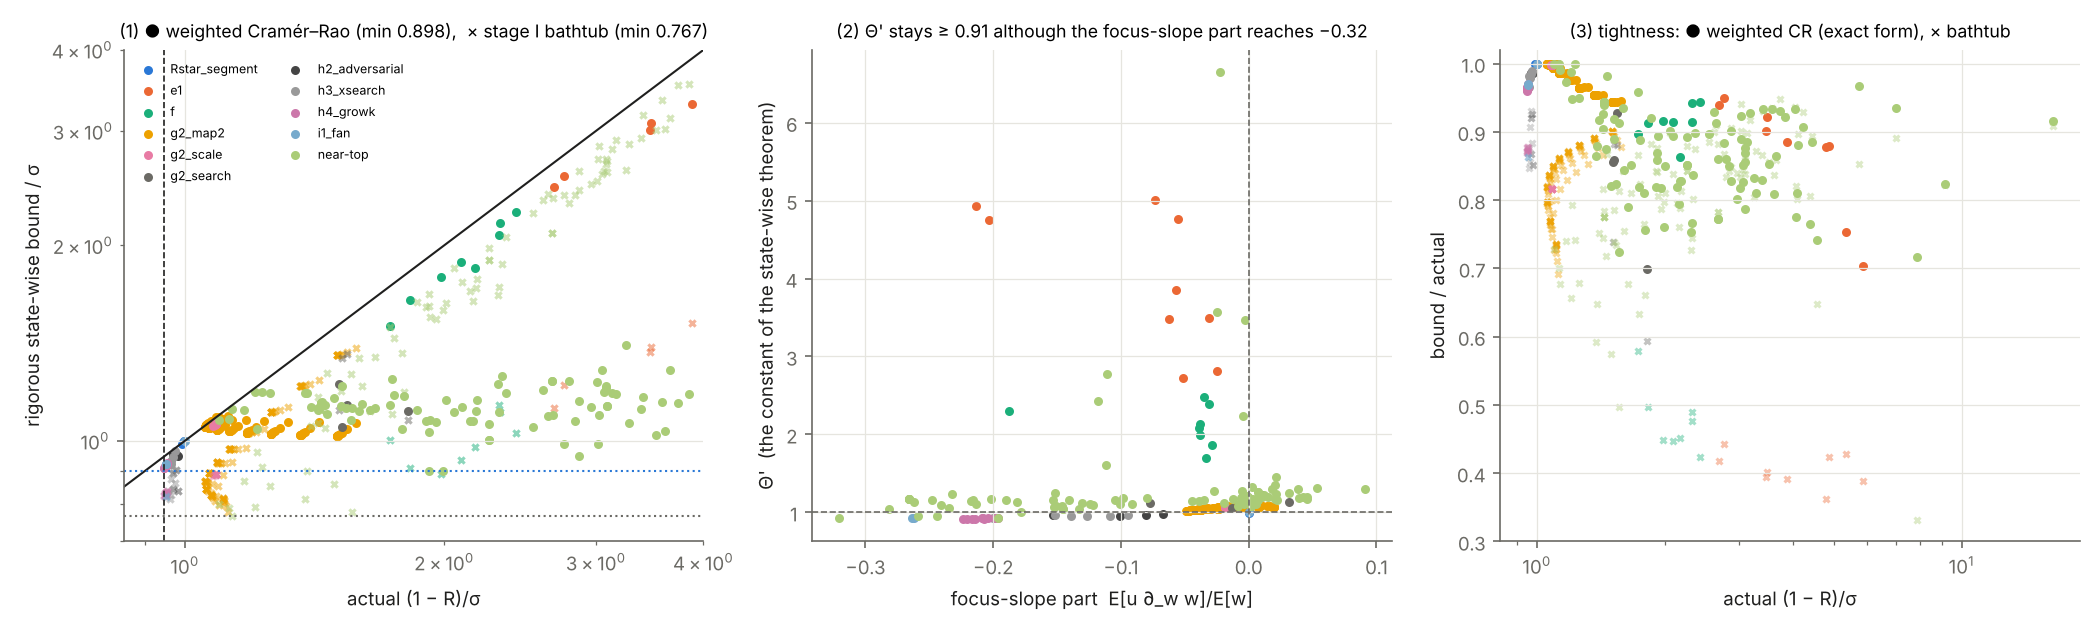
\includegraphics[width=0.95\textwidth]{figures/fig5_bound.png}
\caption{State-wise lower bound for the pendulum. (1) Bound of Theorem~\ref{thm:statewise} (dots) and the earlier, weaker bound that only uses $\omega \leq 1$ (crosses), against the actual gap, for all stored states with $\sigma \leq 10^{-2}$. (2) $\Theta'$ against the focus-slope part of $\E[\omega u s_w]/j$. (3) Ratio of bound to actual gap.}
\label{fig:bound}
\end{figure*}

\begin{observation}[Tightness]
\label{obs:bound}
On all $268$ stored pendulum states with $\sigma \leq 10^{-2}$, including the fans and adversarial states of Sec.~\ref{sec:mixtures}, $\Theta' \geq 0.9125$ and the bound~\eqref{eq:statewise} is at least $0.898\,\sigma$ (Fig.~\ref{fig:bound}). Before the minimization over the auxiliary variable it is at least $0.909\,\sigma$. The smallest actual gap among these states is $0.946\,\sigma$. For the $82$ states with gap below $1.1\,\sigma$ the bound is within $5\%$ of the actual gap.
\end{observation}

What prevents a uniform bound is the following. Integrating by parts along $w$,
\begin{equation}
-\E[\omega u s_w] = \E[\omega\,\partial_w u] + \E[u\,\partial_w\omega] .
\label{eq:ibp}
\end{equation}
The first, geometric term is close to $j$ (at least $0.963\,j$ on all stored states). The second, the \emph{focus slope}, is negative for fans, between $-0.2\,j$ and $-0.3\,j$; it is the mechanism by which mixtures beat the best Gaussian state. Bounding it requires control of $\partial_w H_{vv}$, a third derivative of $\ln\rho_C$, that is, of third posterior cumulants. The bound $H \preceq \sigma^{-2}I$ limits how sharp the focus can be but not how fast it can change, and for mixtures with crossing components the focus can change on short scales. A uniform bound also needs $\tilde\varepsilon + D = o(\sigma)$: $\tilde\varepsilon$ contains the valley term $\E[\gamma[H_{vv}]_-]$, which is not controlled in general, and $D$ can be positive. Numerically both are small near the hyperbolic point ($D/\sigma \leq 0.0022$ for $\sigma \leq 10^{-2}$). Replacing $\omega$ by a weight that is only allowed to vary slowly along $w$ removes the focus slope at the price of a smaller weight (Appendix~\ref{app:bound}, Proposition~\ref{prop:smooth}); under explicit conditions this gives a uniform gap, for example $0.344\,\sigma$ on the stored states concentrated near the hyperbolic point, but the conditions themselves are observed rather than proved.

\section{Numerical evidence and a sharpened conjecture}
\label{sec:evidence}

The results above prove the conjecture of Ref.~\cite{namba2026arrow} for Gaussian states and reduce it, for general states of the pendulum, mainly to a bound on the focus slope. Here we summarize the numerical evidence for the general case. All evaluations are exact up to quadrature error: the posterior moments of Gaussian mixtures are evaluated in closed form, the remaining integrals on adaptive or nested grids, and every reported number was checked against at least one refined grid (Appendix~\ref{app:methods}).

\emph{Searches.} For the pendulum we evaluated random Gaussian mixtures with $K = 2$ to $40$ components, families that vary one parameter at a time, and adversarial searches that maximize $R$, the covariance term, the mass of valleys, the fraction $(R - L)/(\kappa - L)$ of the available room that a state uses, and the advantage $g^*$. Together with the quartic oscillator, the double well and the twist flow, more than $2{,}300$ distinct states were stored and re-evaluated. No state had $R > \kappa$.

\emph{Near the hyperbolic point.} Let $\kappa - L$ be the distance of the law term from $\kappa$. Among states with small distance, the largest excess $R - L$ found decreases at least linearly with the distance: the upper envelope has slope $0.98$ between distances $3\times10^{-4}$ and $3\times10^{-3}$, and $1.26$ over the whole range, and states closer than $3\times10^{-3}$ use at most $9\%$ of the available room. The variance of the local strain $\bar a$ decreases as the square of the distance, because the strain is flat at its maximum, while the focus mismatch $\E\|H - F\|/\tr F$ stays of order one.

\emph{States that use almost all of the room.} The fraction of room used can be pushed towards $1$, but only from below and only through a ruler effect: a needle at $q = \pi$ that carries a small part of the weight but almost all of the Fisher information sets $R$, while a broad component far from the maximum enlarges the distance $\kappa - L$. Along a sequence of shrinking needles we observed that $R$ stays below the critical rate of the needle alone, which is below its strain and below $1$ by Theorem~\ref{thm:gaussian}.

\emph{Gap.} For $\sigma \leq 10^{-2}$ every stored pendulum state has $(1-R)/\sigma \geq 0.946$; the smallest values belong to the fans of Sec.~\ref{sec:mixtures}, whose advantage over the best Gaussian state saturates at about $5\%$ of the Gaussian gap. In the other flows the gap is also proportional to $\sigma$ (Fig.~\ref{fig:flows}).

\begin{figure*}[t]
\centering
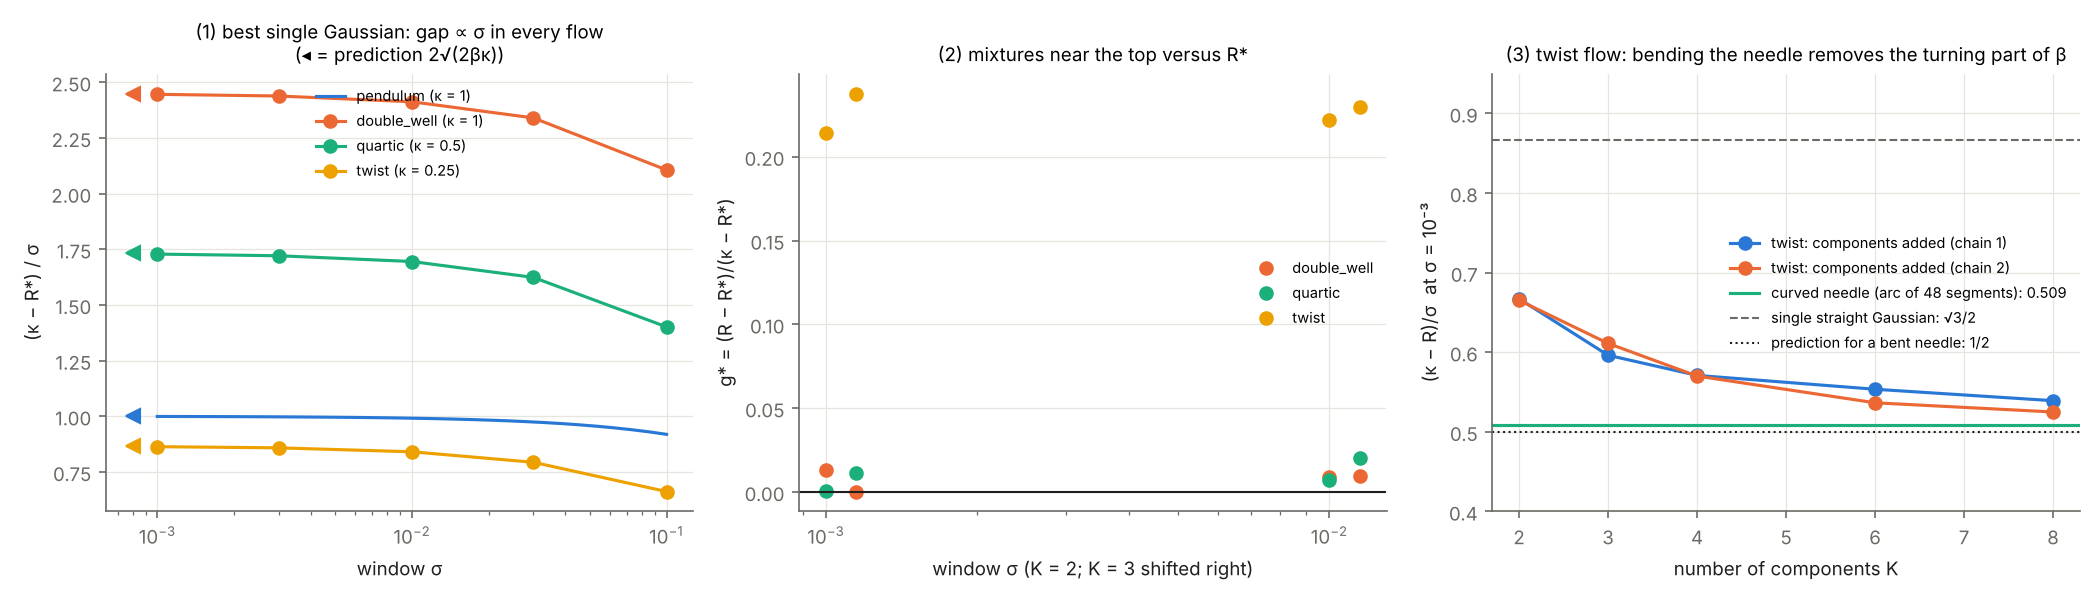
\includegraphics[width=0.95\textwidth]{figures/fig4_flows.png}
\caption{Resolution gap in four flows. (1) Best Gaussian state: $(\kappa - R^*)/\sigma$ against $\sigma$; triangles mark the prediction $2\sqrt{2\beta\kappa}$ of Proposition~\ref{prop:gap}. (2) Advantage $g^*$ of mixtures near the maximal strain. (3) Twist flow: gap of mixtures with $K$ components, of a bent needle, of the best straight Gaussian state ($\sqrt3/2$) and the prediction $1/2$ for a needle that follows the rotation.}
\label{fig:flows}
\end{figure*}

These observations suggest a sharpened form of the conjecture.

\begin{gapconjecture}
For the pendulum there are constants $c > 0$ and $\sigma_0 > 0$ such that every state satisfies $\kappa - R \geq c\,\sigma$ for $\sigma \leq \sigma_0$. Numerically, the best constant is close to $0.95$.
\end{gapconjecture}

The resolution-gap conjecture implies Conjecture~1 of Ref.~\cite{namba2026arrow} for the pendulum at small resolution, with a margin. By Theorem~\ref{thm:statewise} it would follow from a lower bound on $\Theta'$ that holds uniformly over states, together with $\tilde\varepsilon + D = o(\sigma)$. We expect the same structure, a gap $c_f\,\sigma$ with $c_f$ set by the curvature of the strain at its maximum after any rotation of the stretching direction has been followed, for other Hamiltonian flows with finite $\kappa$.

\section{Conclusion}
\label{sec:conclusion}

Whether a coarse-grained entropy can decrease is decided, state by state, by a critical rate $R$. We showed that $R$ splits exactly into a law term that never exceeds the maximal strain $\kappa$, a covariance between the local sharpness of the coarse-grained density and the local strain, and a posterior Stein defect. A violation of $R \leq \kappa$ therefore requires valleys of the coarse-grained density, or non-Gaussian posteriors. For Gaussian states $R \leq \kappa$ holds in any dimension. For one degree of freedom the best Gaussian state is a thin segment through the point of maximal strain, and the finite resolution leaves a gap $2\sqrt{2\beta\kappa}\,\sigma$ to leading order, with an exact series for the pendulum and a closed form for quadratic strain. Mixtures can beat the best Gaussian state, by fans that concentrate the focus at the point of maximal strain and by bent needles that follow a rotating stretching direction, but in all cases examined the gap stays proportional to $\sigma$. For the pendulum, a weighted Cram\'er--Rao inequality gives a lower bound on the gap for every state; it would become uniform with a bound on the speed at which the focus can vary along the contracting direction, together with control of the valleys and of the Stein defect.

The physical content is that imprecision of observation is not only the reason why coarse-grained entropy can grow, but also the reason why its growth is robust: a window of width $\sigma$ cannot be sharper than $\sigma$, and an ensemble that is sharp across the stretching direction must be long along the contracting one. Both effects together keep $R$ a distance proportional to $\sigma$ below $\kappa$. In the limit of perfect resolution the margin closes and the criterion $r \geq \kappa$ of Ref.~\cite{namba2026arrow} becomes marginal.

Three directions remain open. The first is a proof of the resolution-gap conjecture of Sec.~\ref{sec:evidence}, which by Theorem~\ref{thm:statewise} amounts mainly to a bound on how fast the coarse-grained Fisher matrix can vary, probably through a variational argument over all states rather than pointwise estimates. The second is the extension to several degrees of freedom, where stretching directions rotate in general; the twist flow suggests that the relevant curvature is the one that remains after the rotation has been followed. The third concerns generative models. In a diffusion model the local Fisher matrix $H = -\nabla s$ is the Jacobian of the learned score, so the quantities in Eq.~\eqref{eq:where} can be estimated from a trained network. For linear forward drifts the threshold $r = \kappa$ governs which isotropic noise schedules a stochastic differential equation can realize~\cite{namba2026arrow,namba2026threshold}; for nonlinear latent dynamics the decomposition identifies where this threshold can be exceeded.


\appendix
\section{Proofs for Section~\ref{sec:best}}
\label{app:best}

\emph{Reduction to one variable.} Let $\rho_t = \mathcal N(m,S)$ with $\varphi > 0$, so that $S_{ww} > S_{vv}$. Write $d = \sqrt{S_{ww}}$, $\alpha = \sqrt{S_{vv}}$ and $x = d - \alpha > 0$. Positive semidefiniteness gives $S_{vw} \geq -\alpha d$, hence
\begin{equation}
S_{qq} = \tfrac12\left(S_{vv} + 2S_{vw} + S_{ww}\right) \geq \tfrac12 x^2 ,
\label{eq:Sqqmin}
\end{equation}
with equality for the zero-width segment $S_{vw} = -\alpha d$. With $y = d + \alpha$,
\begin{equation}
\varphi = \frac{d^2 - \alpha^2}{d^2 + \alpha^2 + 2\sigma^2} = \frac{2xy}{x^2 + y^2 + 4\sigma^2}
\leq \frac{x}{\sqrt{x^2 + 4\sigma^2}} ,
\label{eq:phibound}
\end{equation}
because, at fixed $x$, the middle expression is maximal at $y^2 = x^2 + 4\sigma^2$, which satisfies $y \geq x$. This proves Eq.~\eqref{eq:phimax}. The optimal segment has $\alpha = (y - x)/2$ and $d = (y + x)/2$; for $\sigma \ll x$, $\alpha \approx \sigma^2/x$ and the tilt angle is $\alpha/d \approx \sigma^2/x^2$.

\emph{Proof of Theorem~\ref{thm:pendulum}.} For the pendulum $\lambda = \tfrac12\left(1 - \cos m_q\,e^{-S_{qq}/2}\right) \in [0,1]$, so states with $\varphi \leq 0$ have $R \leq 0$. For $\varphi > 0$, $\lambda \leq \Lambda(S_{qq})$ with $\Lambda(s) = \tfrac12(1 + e^{-s/2})$, which is decreasing; by Eqs.~\eqref{eq:Sqqmin} and~\eqref{eq:phibound},
\begin{equation*}
R = \lambda\varphi \leq \Lambda(x^2/2)\,\frac{x}{\sqrt{x^2 + 4\sigma^2}} = \frac{1 + e^{-x^2/4}}{2}\,\frac{x}{\sqrt{x^2 + 4\sigma^2}} .
\end{equation*}
Equality holds for the zero-width segment centred at $m_q = \pi$ with the optimal $y$, which proves Eq.~\eqref{eq:Rstar}. As $x \to \infty$ the right-hand side tends to $1/2$ from below; the interior maximum is at least $1/2$ exactly for $\sigma \leq \sigma_c = 0.93909\ldots$ (with equality at $\sigma_c$), obtained numerically from the stationarity condition. For the expansion, put $x^2 = u\sigma$. Then $\Lambda = 1 - u\sigma/8 + O(\sigma^2)$ and $x/\sqrt{x^2 + 4\sigma^2} = 1 - 2\sigma/u + O(\sigma^2)$, so $1 - R = \sigma\,(u/8 + 2/u) + O(\sigma^2)$, minimal at $u = 4$ with value $\sigma$. This gives the length $x \approx 2\sqrt\sigma$ and the tilt $\sigma^2/x^2 \approx \sigma/4$. Expanding the stationarity condition in powers of $\sigma$ gives $u_* = 4 - \sigma + \tfrac58\sigma^2 - \tfrac1{12}\sigma^3 + \cdots$ and, after substitution, the coefficients of Eq.~\eqref{eq:series}; they were computed with exact rational power series up to order $11$.

\emph{Proof of Theorem~\ref{thm:quadratic}.} Here $\lambda = \kappa - b\left[(m_q - q_*)^2 + S_{qq}\right] \leq \kappa - bS_{qq}$. If $\lambda \leq 0$ and $\varphi \geq 0$ then $R \leq 0$. Otherwise, as above, $R \leq \left(\kappa - \tfrac12 bx^2\right)x/\sqrt{x^2 + 4\sigma^2}$, with equality for the centred zero-width segment. Put $x^2 = \sigma\nu\sqrt{\kappa/b}$. Then $\tfrac12 bx^2/\kappa = \varepsilon\nu/2$ and $x^2/(x^2 + 4\sigma^2) = \nu/(\nu + 4\varepsilon)$, so $R/\kappa = (1 - \varepsilon\nu/2)\sqrt{\nu/(\nu + 4\varepsilon)}$. Setting the logarithmic derivative with respect to $\nu$ to zero gives $\nu^2 + 6\varepsilon\nu - 4 = 0$, whose positive root is $\nu = \sqrt{4 + 9\varepsilon^2} - 3\varepsilon$.

\emph{Proof of Proposition~\ref{prop:gap}.} Upper bound on the gap: take the centred zero-width segment with $x^2 = 2\sigma\sqrt{\kappa/b}$ and the optimal tilt. Its $X_q$ is Gaussian with mean $q_*$ and variance $S_{qq} = x^2/2 = O(\sigma)$. By the regularity of $a$ near $q_*$, its polynomial growth, and the vanishing of the odd central moments, $\lambda = \kappa - bS_{qq} + O(S_{qq}^2)$, while $\varphi = 1 - 2\sigma^2/x^2 + O(\sigma^2)$ by Eq.~\eqref{eq:phibound}. Hence $\kappa - R \leq \tfrac12 bx^2 + 2\kappa\sigma^2/x^2 + O(\sigma^2) = 2\sqrt{\kappa b}\,\sigma + O(\sigma^2)$, and $\sqrt{\kappa b} = \sqrt{2\beta\kappa}$. Matching lower bound under the stated condition: as in the proof of Theorem~\ref{thm:pendulum}, and because $\Lambda$ is non-increasing, $R \leq \sup_x \Lambda(x^2/2)\,x/\sqrt{x^2 + 4\sigma^2}$. Because $\sup_{s \geq s_0}\Lambda(s) < \kappa$, the maximizing $x$ tends to $0$ as $\sigma \to 0$; comparing $\kappa - \tfrac12 bx^2(1 + o(1))$ with the achievable $\kappa - O(\sigma)$ shows $x^2 = O(\sigma)$, so that $\Lambda(x^2/2) = \kappa - \tfrac12 bx^2 + O(x^4)$, and the same computation as above shows that the supremum equals $\kappa - 2\sqrt{\kappa b}\,\sigma + O(\sigma^2)$.

\section{Proof of Theorem~\ref{thm:statewise} and a variant}
\label{app:bound}

Write $J = F$, $J_{\rm tot} = \tr F$, $f_0 = L + C$ so that $R = f_0 + D$, and use $(v,w)$ components. For the pendulum $G(y) = \bar a(y)\,\mathrm{diag}(1,-1)$.

\emph{Step 1 (identity).} From $f_0 = \E\tr(HG)/\tr F$ (proof of Proposition~\ref{prop:decomposition}) and $\E H = J$,
\begin{equation}
J_{\rm tot}(1 - f_0) = \E[\gamma H_{vv}] - \E[\gamma H_{ww}] + 2J_{ww}, \qquad \gamma = 1 - \bar a .
\label{eq:step1}
\end{equation}

\emph{Step 2 (positive and negative parts).} $\E[\gamma H_{vv}] = \E[\gamma\omega]/\sigma^2 - N$ with $N = \E[\gamma\,[H_{vv}]_-]$.

\emph{Step 3 (strain inequality).} For all real $x$, $\cos x \leq 1 - x^2/2 + x^4/24$, so $\sin^2(x/2) \geq x^2/4 - x^4/48$. Averaging over the posterior and using $\E[\delta^2\,|\,y] = u^2/2 + \Var(X_q\,|\,y)$,
\begin{equation}
\gamma \geq \frac{u^2}{8} + \frac{\Var(X_q\,|\,y)}{4} - \frac{\E[\delta^4\,|\,y]}{48} .
\end{equation}

\emph{Step 4 (weighted Cram\'er--Rao).} Since $\omega \geq 0$, the Cauchy--Schwarz inequality gives $\E[\omega u^2] \geq \Gamma^2/\E[\omega s_w^2]$ with $\Gamma = -\E[\omega u s_w]$. For $\omega \equiv 1$, integration by parts gives $\Gamma = \E[\partial_w u]$ and this is the Cram\'er--Rao inequality along $w$.

\emph{Step 5 (window bound).} By Eq.~\eqref{eq:Hbound}, $0 \leq \omega \leq 1$ and $J_{vv} = \E[H_{vv}] \leq \E[[H_{vv}]_+] = j/\sigma^2$, so $J_{\rm tot} \leq j/\sigma^2 + J_{ww}$.

\emph{Step 6 (combination).} Steps 1--4 give $J_{\rm tot}(1 - f_0) \geq \mathcal P - \mathcal Q$ with
\begin{align*}
\mathcal P &= \frac{\Gamma^2}{8\sigma^2\E[\omega s_w^2]} + 2J_{ww} \geq 0, \\
\mathcal Q &= \frac{\E\!\left[\omega\left(\tfrac{1}{48}\E[\delta^4|Y] - \tfrac14\Var(X_q|Y)\right)\right]}{\sigma^2} + N + \E[\gamma H_{ww}] .
\end{align*}
Divide by $J_{\rm tot}$. Because $\mathcal P \geq 0$, Step 5 gives $\mathcal P/J_{\rm tot} \geq \mathcal P/(j/\sigma^2 + J_{ww})$; the remainder is divided exactly, $\mathcal Q/J_{\rm tot} = \tilde\varepsilon$. With $\Theta'$ from Eq.~\eqref{eq:Theta} and $\zeta = \sigma^2 J_{ww}/j$,
\begin{equation}
1 - f_0 \geq \frac{\Theta'^2\sigma^2/(8\zeta) + 2\zeta}{1 + \zeta} - \tilde\varepsilon .
\end{equation}

\emph{Step 7 (minimization).} Let $T = \Theta'\sigma$. For $\zeta \leq T/2$, the arithmetic--geometric mean inequality gives $T^2/(8\zeta) + 2\zeta \geq T$, hence the fraction is at least $T/(1+\zeta) \geq T/(1 + T/2)$. For $\zeta > T/2$ the fraction is at least $2\zeta/(1+\zeta) \geq T/(1 + T/2)$. (The split is not optimal; the exact minimum over $\zeta$ exceeds $T/(1+T/2)$ only by $O(T^2)$.)

\emph{Step 8.} $1 - R = 1 - f_0 - D$, which proves Eq.~\eqref{eq:statewise}. Only the inequalities of Steps 3, 4, 5 and 7 were used, and none of them needs a sign condition. (Dividing the whole right-hand side of Step 6 by $j/\sigma^2 + J_{ww}$ would require $\mathcal P - \mathcal Q \geq 0$; the split above avoids this.)

\emph{A variant with a slowly varying weight.} The focus-slope term of Eq.~\eqref{eq:ibp} enters through $\Gamma$. It can be removed by replacing $\omega$ with a smaller weight whose variation along $w$ is limited. For $M > 0$ let $\chi$ be the largest function with $0 \leq \chi \leq \omega$ such that $\sqrt\chi$ is $(M/2)$-Lipschitz along $w$; then $|\partial_w\chi| \leq M\sqrt\chi$, and $\E[\gamma\omega] \geq \E[\gamma\chi]$ because $\gamma \geq 0$.

\begin{proposition}[Slowly varying weight]
\label{prop:smooth}
Let $M = m\sqrt{J_{ww}}$ with $m > 0$, and define $j_\chi = \E\chi$, $\mu = j_\chi/j$ (the fraction of the focus weight that survives), $G_\chi = \E[\chi\,\partial_w u]/j_\chi$, $\pi_\chi = \Pr[\chi(Y) > 0]$, $\kappa_2 = 2 - \E[\gamma H_{ww}]/J_{ww}$ and
\begin{equation*}
\varepsilon_2 = \frac{1}{J_{\rm tot}}\left\{\frac{\E\!\left[\chi\left(\tfrac1{48}\E[\delta^4|Y] - \tfrac14\Var(X_q|Y)\right)\right]}{\sigma^2} + N\right\}.
\end{equation*}
With $\Theta_\chi = \mu\,[G_\chi]_+/(1 + m\sqrt{\pi_\chi})$ and $T = \Theta_\chi\sigma\sqrt{\kappa_2/2}$, every state of the pendulum with $\kappa_2 > 0$ satisfies
\begin{equation}
1 - R \geq \frac{T}{1 + T/\kappa_2} - \varepsilon_2 - D .
\end{equation}
\end{proposition}

\begin{proof}
With $Z = \E[\chi u^2]$, Cauchy--Schwarz and integration by parts give $\sqrt Z\sqrt{\E[\chi s_w^2]} \geq |\E[\chi\,\partial_w u] + \E[u\,\partial_w\chi]|$, and $|\E[u\,\partial_w\chi]| \leq M\,\E[|u|\sqrt\chi] \leq M\sqrt{Z\pi_\chi}$. Since $\E[\chi s_w^2] \leq J_{ww}$, this gives $\sqrt Z \geq j_\chi[G_\chi]_+/\bigl(\sqrt{J_{ww}}\,(1 + m\sqrt{\pi_\chi})\bigr)$. Keeping $-\E[\gamma H_{ww}] + 2J_{ww} = \kappa_2J_{ww}$ in the positive part and repeating Steps 5--7 with $\kappa_2$ in place of $2$ gives the claim; in Step 7 the two regimes are separated at $\zeta = T/\kappa_2$.
\end{proof}

With $m = 1$ the variant gives at least $0.389\,\sigma$ on the $236$ stored states concentrated near the hyperbolic point, where $\mu \geq 0.814$, $G_\chi \geq 0.974$, $\kappa_2 \geq 1.967$ and $\varepsilon_2 + D \leq 0.049\,\sigma$; with these constants the bound is $0.344\,\sigma$ uniformly on that class. The lower bounds on $\mu$, $G_\chi$ and $\kappa_2$ are observed, not proved. Restricting the number or the width of the components does not imply them, because two crossing components can already make the focus vary on arbitrarily short scales.

\section{Numerical methods and independent checks}
\label{app:methods}

\emph{Evaluator.} All states are Gaussian mixtures $\rho_t = \sum_k w_k\mathcal N(m_k,S_k)$. The coarse-grained density, its score and $H$ are then mixtures in closed form, and so are the posterior moments that enter $\Sigma$, $G$ and $D$: for the pendulum $\E[\sin X_q]$ and $\E[\cos X_q]$ under a Gaussian are elementary. Only the final integrals over $y$ are done by quadrature, on uniform grids aligned with $(v,w)$. Thin components (``needles'') are handled by nested grids: a smooth partition of unity refines the grid near each needle, the total mass is reproduced to $10^{-12}$, and further refinement changes $R$ by less than $10^{-9}$. Every reported state was re-evaluated on a refined grid.

\emph{Independent evaluations.} The central numbers were reproduced by methods that do not use the closed-form posterior moments of the evaluator; methods (iii) and (iv) were also written separately from the evaluation code.
(i)~Gauss--Hermite quadrature of the posterior expectations instead of closed forms ($10^{-14}$).
(ii)~Direct summation over quadrature nodes of each component, with the Gaussian kernel and its derivatives summed explicitly ($5\times10^{-8}$ for the mixtures that beat the best Gaussian state).
(iii)~The entropy itself, without any of the identities of Sec.~\ref{sec:decomposition}: the fine-grained density is transported exactly by the flow over $\pm\,\Delta t$ (fourth-order Runge--Kutta for the characteristics), blurred with the Gaussian window either by fast Fourier transform on a grid or by summing kernels over transported nodes, and $\Sigma$ is obtained from the central difference of $S_C$. With this method we reproduced $R$ for pendulum mixtures to five digits ($0.31498$, $0.33255$, $0.33116$), the state with $R = 0.98545$ to $4\times10^{-5}$, the two violations of $R \leq R^*$ in Sec.~\ref{sec:mixtures} to $10^{-7}$, and the best $K = 8$ state of the twist flow to $4\times10^{-10}$.
(iv)~The best Gaussian state was obtained independently by direct optimization of Eq.~\eqref{eq:lambdaphi} over all Gaussian states, in agreement with Eq.~\eqref{eq:Rstar} to twelve digits.

\emph{Verification suite.} Each stage of the numerical study has a script that re-derives every number it reports from stored raw results and checks the identities used (for example Eq.~\eqref{eq:decomposition} to $10^{-11}$, the second-order Tweedie formula, Step~1 of Appendix~\ref{app:bound} to $10^{-15}$, and the inequalities of Steps 3--7 on every state). In total the suite contains 281 checks; each check reports the fraction of its tolerance that it uses, and none uses more than $20\%$.


\section*{Acknowledgments}
The author used two AI assistants in this work: Google Gemini (\mbox{Gemini 3.8 Flash}), for independent cross-checking of the derivations and results from several angles; and Anthropic Claude (\mbox{claude-opus-5-5}), in two separate sessions. In the first session it took part in theoretical discussion, proposed and checked proofs, derived the one-variable form~\eqref{eq:Rstar}, wrote independent numerical checks, and drafted and edited the text of the manuscript. In the second session it designed and ran the numerical study, wrote the evaluation and verification code, derived Theorem~\ref{thm:statewise}, Proposition~\ref{prop:smooth}, the closed form~\eqref{eq:quadratic} and the series~\eqref{eq:series}, and generated the figures. Results were passed between the sessions as written summaries, and every summary was checked in the first session by re-running the full verification suite and, for the central numbers, by the independent methods of Appendix~\ref{app:methods}. The instructions given to the assistants consisted of the author's research questions and requests to derive, check, critique, compute or rephrase specific results. Several turns of the study were proposed by the author: to observe the nonlinear problem numerically before attempting a proof, to examine the spatial spread of the local anisotropy, which identified the covariance term as the mechanism of excess over single components, to ask whether the flow singles out a reference frame, which led to the formulation in the stretching and contracting directions, to follow the rotation of that frame in flows where it turns, and to report the refutation of the extremality of Gaussian states as a result in its own right. No result was adopted without verification: every analytical statement, number and figure was checked against independent numerical evaluation in the openly available code, and all bibliographic information was checked against the original sources. The author directed the research, made all decisions on its content, and takes full responsibility for this article.

\section*{Data and Code Availability}
Scripts that reproduce every analytical statement, number and figure of this article, together with the verification suite, are openly available at \url{https://github.com/neginyan/resolution-gap-arrow-of-time}. The version used for this article is archived at Zenodo, doi:~[to be assigned].


\begin{thebibliography}{99}

\bibitem{gibbs1902}
J.~W.~Gibbs, \textit{Elementary Principles in Statistical Mechanics} (Charles Scribner's Sons, New York, 1902).

\bibitem{ehrenfest1912}
P.~Ehrenfest and T.~Ehrenfest, \textit{The Conceptual Foundations of the Statistical Approach in Mechanics} (Cornell University Press, Ithaca, 1959); original German edition 1912.

\bibitem{wehrl1978}
A.~Wehrl, Rev. Mod. Phys. \textbf{50}, 221 (1978).

\bibitem{lebowitz1993}
J.~L.~Lebowitz, Phys. Today \textbf{46}(9), 32 (1993).

\bibitem{namba2026arrow}
T.~Namba, \textit{Sharp criterion for the coarse-grained arrow of time in Hamiltonian dynamics}, preprint, version v1.1.1, Zenodo (2026), \href{https://doi.org/10.5281/zenodo.23163727}{doi:10.5281/zenodo.23163727}.

\bibitem{efron2011}
B.~Efron, J. Am. Stat. Assoc. \textbf{106}, 1602 (2011).

\bibitem{hamilton1993}
R.~S.~Hamilton, Commun. Anal. Geom. \textbf{1}, 113 (1993).

\bibitem{stein1981}
C.~M.~Stein, Ann. Stat. \textbf{9}, 1135 (1981).

\bibitem{sarkka2013}
S.~S\"arkk\"a, \textit{Bayesian Filtering and Smoothing} (Cambridge University Press, Cambridge, 2013).

\bibitem{stam1959}
A.~J.~Stam, Inf. Control \textbf{2}, 101 (1959).

\bibitem{cover2006}
T.~M.~Cover and J.~A.~Thomas, \textit{Elements of Information Theory}, 2nd ed. (Wiley, Hoboken, 2006).

\bibitem{rao1945}
C.~R.~Rao, Bull. Calcutta Math. Soc. \textbf{37}, 81 (1945).

\bibitem{cramer1946}
H.~Cram\'er, \textit{Mathematical Methods of Statistics} (Princeton University Press, Princeton, 1946).

\bibitem{namba2026threshold}
T.~Namba, \textit{A stretching-rate threshold for phase-space diffusion models with isotropic marginal noise schedules}, preprint, Zenodo (2026), \href{https://doi.org/10.5281/zenodo.23181225}{doi:10.5281/zenodo.23181225}.

\end{thebibliography}


\end{document}
